\documentclass[a4paper,12pt]{article}
\usepackage{header}
\usepackage{enumitem}
\providecommand{\keywords}[1]
{
  \small	
  \textbf{\textit{Keywords---}} #1
}

\begin{document}
\selectlanguage{russian}

    
\large
\bigskip

\begin{center}
{\large Федеральное государственное автономное образовательное 

учреждение высшего образования

Национальный исследовательский университет

\smallskip

<<Высшая школа экономики>>

}

\bigskip
\bigskip
\bigskip

{ \large
Факультет компьютерных наук

Основная образовательная программа

Прикладная математика и информатика
}
\end{center}

\begin{center}
  {\large Выпускная квалификационная работа}
  
  {\large на тему}
\end{center}

\begin{center}
  \textbf{\huge Распознование именованных сущностей для языков с малыми ресурсами}
\end{center}


\renewcommand{\arraystretch}{1.8} %% increase table row spacing

\bigskip
\bigskip
\bigskip
\bigskip

{\large Выполнила студентка группы БПМИ151, 4 курса,

\hspace{3cm} Закирова Ксения Игоревна


Научный руководитель:

\hspace{3cm} Доцент, кандидат технических наук,

\hspace{3cm} Артемова Екатерина Леонидовна


}
    
\bigskip
\bigskip

\bigskip
\bigskip
\bigskip
\pagestyle{empty}

\vfill
\begin{center}
  {Москва, 2020}
\end{center}

\newpage
    \pagestyle{empty}
    \tableofcontents
    \pagestyle{plain}
    
\newpage    
    
\selectlanguage{english}
\begin{abstract}
In this work, I investigate the approaches to the problem of named entity recognition in the Tatar language, The Tatar language is low-resource, so I tackled both initial data collection and modelling. I automatically annotated corpora from Tugan Tel and Wikipedia and I present a list of named entities. Corpora contain labels such as PER, LOC, ORG and MISC in BIO notation. I train BiLSTM-CRF and BERT models. The BERT-based model achieves 0.47 average F-score. 
\end{abstract} \hspace{10pt}

%TC:ignore
\keywords{Named Entity Recognition, NER, Tatar language, low-resource languages}
%TC:endignore
\selectlanguage{russian}

\begin{abstract}
В данной работе я рассмотрела задачу извлечения именованных сущностей в татарском языке, собрала данные для корпуса Википедии и обучила машинную модель. Татарский является малоресурсным языком, для которого нет доступных решений в литературе. Результатом работы является список именованных сущностей и размеченный с помощью алгоритма корпус на основе Википедии, который я предоставляю в открытый доступ. Корпус содержат теги PER, LOC, ORG и MISC в нотации BIO. Я обучила модели BiLSTM-CRF и BERT. BERT показал средний результат метрики f-score 0.47 на тестовом наборе, который был размечен вручную
\end{abstract} \hspace{10pt}

    \section{Введение}

Извлечение именованных сущностей (Named entity recognition, NER) это одна из задач обработки естественного языка; задача обнаружения и классификации слов в тексте на несколько заранее определённых категорий, таких как, имена, люди, географические названия, организации и т.д. На вход подаётся текст (предложение), на выходе --- массив из меток для каждого слова (словоформы -- слова, знаки препинания, числа, прочие сущности, которые есть в тексте).

\begin{table}[h]
\begin{tabular}[h]{ccccccccccc}
\textcolor{green}{B-PER} & \textcolor{green}{I-PER} & O & O & \textcolor{blue}{B-ORG} &  \textcolor{blue}{I-ORG} &  \textcolor{blue}{I-ORG} & O & \textcolor{red}{B-TIM} & O & O \\
Иван & Петров & преподает & в & Высшей & Школе & Экономики & с & 2014 & года & . \\
\end{tabular}
\caption{Пример размеченных данных, использована нотация BIO}
\end{table}

Извлечение именованных сущностей имеет множество применений: в автоматическом разделении на категории текстов, в рекомендательных системах, в системах извлечения информации. Как задача извлечение именованных сущностей была сформулирована ещё в 1996 году \cite{first_NER}, однако широкое распространение получила только в последнем десятилетии \cite{DBLP:journals/corr/abs-1812-09449}. Развитие глубоких нейронных сетей дало значительный толчок развитию обработке естественных языков, и, как следствие, задаче извлечения именованных сущностей. Были изобретены более эффективные и точные модели, которые показывают хорошие результаты. Однако остаются и нерешенные проблемы, связанные с данной задачей. Во-первых, упомянутые выше модели с хорошими результатами существуют только для широко распространённых языков, для которых имеются размеченные корпусы, а языки, которые не входят в <<топ-10>> по числу носителей, оказываются вне внимания исследователей. Во-вторых, у компаний и исследователей недостаточно причин прикладывать усилия к задаче извлечения именованных сущностей для языков с малыми ресурсами, так как, скорее всего, это не сможет принести большой выгоды в дальнейшем из-за сравнительно небольшого числа носителей. У меня есть причина личного характера: татарский язык является родным языком для меня, и я стараюсь сохранять и развивать его, в том числе и с помощью этой работы.

Помимо патриотических мотивов есть и прагматические мотивы: развитие извлечение именованных сущностей для татарского языка может быть использовано для всей кыпчакской группы тюркской ветви языков (татарский, башкирский, карачаево-балкарский, казахский, киргизский и др.). Это связано с тем, что языки тюркской ветви достаточно похожи между собой, как грамматически, так и лексически. Как следствие, решение задачи для одного языка скорее всего будет иметь неплохие шансы и для других языков данной группы. К сожалению, это не сработает для турецкого языка, во-первых, потому что он относится к огузской группе, во-вторых (и это главная причина): там используется другой алфавит. Тюркская ветвь включает себя языки с различной письменностью, что усложняет возможность экстраполяции модели на <<похожие>> языки. %TODO найди ссылку!!!

Работа \cite{Nevzorova} исследователей из Академии наук Республики Татарстан даёт рекомендации к разметки корпуса. Далее я более подробно рассмотрю их работу в своем исследовании.

Целью работы является получить размеченный корпус и обученную модель, распознающую именованные сущности и сравнить полученные результаты с ранее имеющимися в этом поле. Работа содержит в себе обзор литературы, получение и разметку данных, выбор двух текущих лучших моделей, обучение моделей и экспериментальную оценку. Поставленная задача формулируется следующим образом: получить систему, на вход которой можно подать текст (предложение) и на выход получить данный текст с тегами для каждой сущности, входящей в этот текст.













    \section{Обзор литературы}

На данный момент существует одна релевантная моему исследованию статья про работу конкретно в татарском языке, однако она не содержит в себе использование методов современного машинного обучения. Также есть работы на темы других языков с малыми ресурсами и работы о моделях, которые были полезны в моей работе.

\subsection{Named Entity Recognition in Tatar: Corpus-Based Algorithm}

Самая близкая к моей работе это статья <<Named Entity Recognition in Tatar:
Corpus-Based Algorithm>> от О. Невзоровой, Д. Мухамедшина и А. Галиевой, Академия наук Республики Татарстан. В статье они рассказывают, как разметили корпус <<Туган Тел>>[ссылка], использовав следующие категории: книги, рестораны, фильмы, журналы, компании, аэропорты, корпорации, языки, колледжи, университеты, школы, магазины, музеи и больницы. Несмотря на наличие в названии распознавания именованных сущностей, они скорее использовали полуручной метод разметки. 

TODO сделай везде доллары, где есть математика!!!

TODO Тут будет описание их статьи.

TODO Куда вставить описание Туган Тел?

\subsubsection{Использованные данные}

Туган Тел -- это корпус текстов на татарском языке, разработанный Институтом прикладной
семиотики Академии наук Республики Татарстан. Корпус предназначен для широкого круга 
пользователей: лингвистов, специалистов в татарском языке, преподавателей татарского и всем 
тем, кому может понадобиться набор текстов на татарском языке. Основными функциями корпуса 
являются: поиск  по словоформе, лемме (лексеме), набору морфологических параметров. 
Существует система <<корпус-менеджер>>, которая поддерживает данные функции.  На данный 
момент существует проект разработки электронного корпуса, который также включает в себя 
автоматическую разметку корпуса, чем и занималась команда Невзоровой. Корпус включает в 
себя татарские тексты различных жанров, такие как художественная литература, тексты СМИ, 
тексты официальных документов, учебная литература, научные публикации и др. Каждый
документ имеет метаописание, включающее в себя автора и его пол, выходные данные, дату 
создания, жанр, части, главы и др. Тексты, включенные в корпус, снабжены автоматической 
морфологической разметкой, которая включает в себя информацию о части речи и 
грамматической характеристики словоформы. Морфологическая разметка текстов корпуса 
выполняется автоматически с использованием модуля двухуровневого морфологического анализа 
татарского языка, реализованного в программном инструментарии PC-KIMMO, с чем связан ряд 
проблем в использовании данного корпуса, о которых я скажу в основной части работы. На 
декабрь 2019 года в корпусе 194 млн. словоформ. 

TODO Нужен ли этот абзац или нафиг его надо?

В качестве релевантных статей Невзорова at al указывают LingPipe[ссылка], команда которой 
решает похожую задачу в английском языке (TODO проверить, так ли это, и о чём вообще статья), 
Annie[ссылка], Afner[ссылка], ссылаются также на марковские цепи, решающие деревья и CRF,
которые потом не используют (в то время как я в этой работе использую). В общем, много хороших 
разных ссылочек, которые надо изучить подробнее, чтобы что-нибудь про них написать. Или вырезать это всё в целом.

\subsubsection{Разбор алгоритма, предложенного в статье:}

Представленный алгоритм основан на идее сравнения $n$-грамм. Сравнение происходит на всём 
объёме корпуса, что увеличивает точность результата, заявляют авторы статьи. Алгоритм является итеративным, причём количество итераций определяется пользователем (что показывает, что их алгоритм является в некоторой степени полуручным.

Первым шагом алгоритма включает в себя выборку по поисковому запросу. Запрос может 
представлять собой форму слова, лемму, фразу или поиск по морфологическим параметром. 
Выборка представляет собой набор биграмм и их количество вхождений в текст. В биграмме одно 
слово является запросом, в то время как второе слово может добавляться слева или справа, данный 
параметр выбирается пользователем. Полученный список биграмм отсортировывается по частоте 
вхождений в корпус и в выборке остаются только самые частотные (например, первые 95\%, в статье 
этот параметр обычно был равен 80\%). Порог отсечения (в статье он называется <<индекс 
покрытия>>, <<covering index>>) более частотных вхождений также выбирается пользователем. 
Урезанный по порогу список биграмм используется как входные данные для второй итерации 
алгоритма: каждая биграмма ищется по корпусу как фраза и, аналогично первому шагу, 
составляются триграммы и их частоты. Точно так же выбираются самые частотные триграммы 
(третье слово может добавляться справа или слева), список обрезается по пороговому значению и,
при желании, алгоритм продолжается дальше, используя на вход уже список триграмм.

Таким образом алгоритм использует $n$-граммы для поиска $(n+1)$-грамм, некоторые из которых будут отсечены порогом, а остальные использованы в следующем шаге алгоритма.

\subsubsection{Окончание алгоритма:}

Существует такое понятие как <<точность сравнения>> (<<accuracy of matching>>) $P$, которое задаётся пользователем в процентах. Если частота $n$-граммы меньше $P$ от количества найденных $(n+1)$-грамм, то $n$-грамма считается именованной сущностью, иначе алгоритм переходит на следующую итерацию. Таким образом, в финальный результат входят самые стабильные $n$-граммы разной длины, включая результаты поиска изначального поискового запроса.

Запрос извлечения именованных сущностей представляет собой кортеж (1), где $Q_1$ и $Q_2$ никак не объясняются, $L, R$ это, соответственно, порог ограничения итераций добавления слов слева и справа, $C$ --- порог отсечения частотности на каждой итерации (covering index), $P$ --- порог для принятия решения о включении фразы в итоговый список именованных сущностей (accuracy of matching). В качестве примера они снова ссылаются на формулу (1) (скорее всего, имелась в виду формула (2) из примера).


\[Q = (Q_1, Q_2, L, R, C, P)\]

\subsubsection{Эксперименты:}

Тут, конечно, всё хитро: выставляются, естественно, только те результаты, где всё получилось хорошо, а где получилось не слишком хорошо --- об этом ничего не сказано. Исследователи перечисляют довольно много категорий, над которыми они экспериментировали, но результаты они показали на словах <<министерство>>, <<улица>>, <<язык>>, <<ресторан>> и <<корпорация>>. Одной из очевидных дополнительных тем являлись бы <<реки>>, но Невзорова at al. на реках экспериментировать не стали.

Также в данной статье очень интересный способ оценки результатов. Стандартные accuracy, precision и recall (и производная от них F-score) в статье не упоминается, к сожалению, но по тексту можно вычленить нечто на них похожее. 

TODO А мне вообще нужна эта статья в обзоре литературы? Я в итоге вообще ничего из неё не взяла.

\subsection{Low-Resource Named Entity Recognition with Cross-Lingual, Character-Level Neural Conditional Random Fields}

https://www.aclweb.org/anthology/I17-2016.pdf

Статья от Ryan Cotterell и Kevin Duh, где представлена модель Conditional Random Fields (CRF)[TODO ссылка?] и представлены способы её улучшения с помощью таких надстроек, как обучение модели на языках с бОльшими ресурсами, а потом применение её к языку из того же семейства, но с меньшими ресурсами. К сожалению, в текущей работе применить данную модель не удалось, но в будущих работах можно опробовать её на тюркской группе языков. В работе от Ryan Cotterell и Kevin Duh рассматривались семья индоевропейских, ветви: романская, германская, славянская, индоарийская; и семья автронезийских, ветвь: филиппинская. Татарский язык относится к тюркской семье, но в то же время существует известная проблема классификации тюркских языков 
%[ссылка https://ru.wikipedia.org/wiki/Классификация\_тюркских\_языков]
TODO релевантность?
что усложняет использование моделей подобного рода.

\subsection{A Neural Layered Model for Nested Named Entity Recognition}
https://www.aclweb.org/anthology/N18-1131.pdf

Статья от Meizhi Ju, Makoto Miwa и Sophia Ananiadou. В данной работе представляется модель Layered-BiLSTM-CRF, которую я использовала в своей работе.

TODO насколько подробно мне нужно в это углубляться? Нужно ли здесь расписывать архитектуру модели, или надо сделать это в основной части?

Исследователи представляют модель, которая работает с <<наслоенными>> именованными сущностями, т.е. когда одна именованная сущность частично или полностью входит в другую именованную сущность. В конечном итоге мои данные не имеют таких наслоений, так что, можно сказать, что данная модель является излишеством, но, как показали эксперименты, она неплохо работает и для <<однослойной>> разметки.

TODO Наверное, что-то ещё надо?

\subsection{Datasets and Baselines for Named Entity Recognition in Armenian Texts}

Очень вдохновляющая статья (вообще говоря, магистерская работа), которая, по факту, и стала решающей при выборе темы. Тема моей работы очень близка к теме работы данных исследователей, за исключением языка: у них, как понятно из названия, армянский язык, который так же относится к языкам малой языковой группы.

В отличие от моего случая, где существует релевантная работа, поднимавшая раньше тему моей работы, Т. Гукасян, Г. Давтян, К. Аветисян и И. Андрианов стали, можно сказать, первопроходцами в своей области, поскольку никто не делал подобных работ для армянского языка. У них не было подобранного и размеченного корпуса текста, поэтому, помимо распознавания именованных сущностей, они занимались также и сбором и разметкой данных. Их модель включала в себя CRF, которую я использую и в своей работе, и рекомендую как хорошую модель для языков с малыми ресурсами.

В своей работе исследователи не использовали BERT, поскольку это относительно новая модель, а статья вышла в конце 2018 года. У меня, к счастью, такая возможность есть, поэтому я ей воспользовалась.

\subsection{BERT: Pre-training of Deep Bidirectional Transformers for
Language Understanding}
https://arxiv.org/pdf/1810.04805.pdf

Данная статья от Google AI Language, которая на текущий момент является state-of-the-art моделью практически на всех популярных бенчмарках обработки естественного языка. Она включает в себя очень много возможностей для различных задач NLP, которые на данный момент пользуются большой популярностью. Для конкретно моей задачи очень хорошо подходит претренированная модель bert-base-multilingual-cased, в обучающие данные которой входила также и Википедия на татарском языке.

Несмотря на популярность BERT, даже дообучать данную модель довольно сложно из-за её размеров. Спасибо Высшей Школе Экономики за возможность использования кластера для обучения моделей для выпускной квалификационной работы.

BERT --- это очень большая модель, которая, однако, не решает задачи распознования именованных сущностей сама по себе, поэтому я воспользовалась библиотекой transformers от huggingface [ссылка https://huggingface.co/transformers/index.html]

\subsection{Huggingface Transformers}

Данная библиотека предоставляет возможность использовать различные state-of-the-art модели (не только BERT, но и многие другие) для решения различных задач обработки естественного языка, в том числе и распознование именованных сущностей, что и является моей задачей.
Их репозиторий на github [ссылка https://github.com/huggingface/transformers] содержит множество примеров [ссылка https://github.com/huggingface/transformers/tree/master/examples/] для удобного использования их библиотеки. Я воспользовалась их библиотекой для решения поставленной задачи распознавания именованных сущностей в татарском языке.







    \section{Методология}

Целью работы было получить размеченный корпус и обученную модель, извлекающую именованные сущности. После обзора литературы были намечены задачи, и работа была предварительно разделена на несколько этапов.

\begin{enumerate}
\item Получение и разметка данных
\item Выбор, обучение и тюнинг моделей
\item Сравнение результатов
\end{enumerate}

Но в ходе работы в план были внесены корректировки. Во-первых, как я упоминала ранее в обзоре литературы, представленные в статье Невзоровой результаты невозможно сравнивать с моими, поскольку постановка задач в моей и их работах различаются. Во-вторых, качество полученных данных оказалось не лучшим из возможных, а алгоритм Невзоровой, разработанный как раз для разметки данных, мог бы улучшить разметку корпуса, используемого для обучения моделей. Как следствие, было принято решение воспроизвести алгоритм из статьи Невзоровой и воспользоваться полученными результатами для разметки данных.

\begin{enumerate}
\item Получение и конвертирование данных в нужный формат.
\item Выбор, обучение и тюнинг моделей
\item Воспроизведение статьи Невзоровой
\item Разметка данных с помощью алгоритма Невзоровой
\item Обучение и тюнинг моделей
\item Сравнение результатов
\end{enumerate}


\section{Получение и разметка данных}

\subsection{Туган Тел}

Обзор литературы показал, что существует корпус татарских текстов Туган Тел\cite{tugan_tel}. Данный корпус имеет систему <<корпус-менеджер>>, которая представлена в виде сайта. На этом сайте можно искать по словоформе или лемме с огромным количеством параметров [\ref{fig:tugan_tel_1}], однако возможности просто скачать весь корпус не оказалось. Я предполагаю, что у Академии наук Республики Татарстан есть API для исполнения запросов на большом количестве данных и в каком-то более удобном формате, чем запрос на сайте, но у меня доступа к такому ресурсу не было.

\begin{figure}
\caption{Параметры на сайте \href{http://tugantel.tatar/}{tugantel.tatar} для поиска по корпусу}
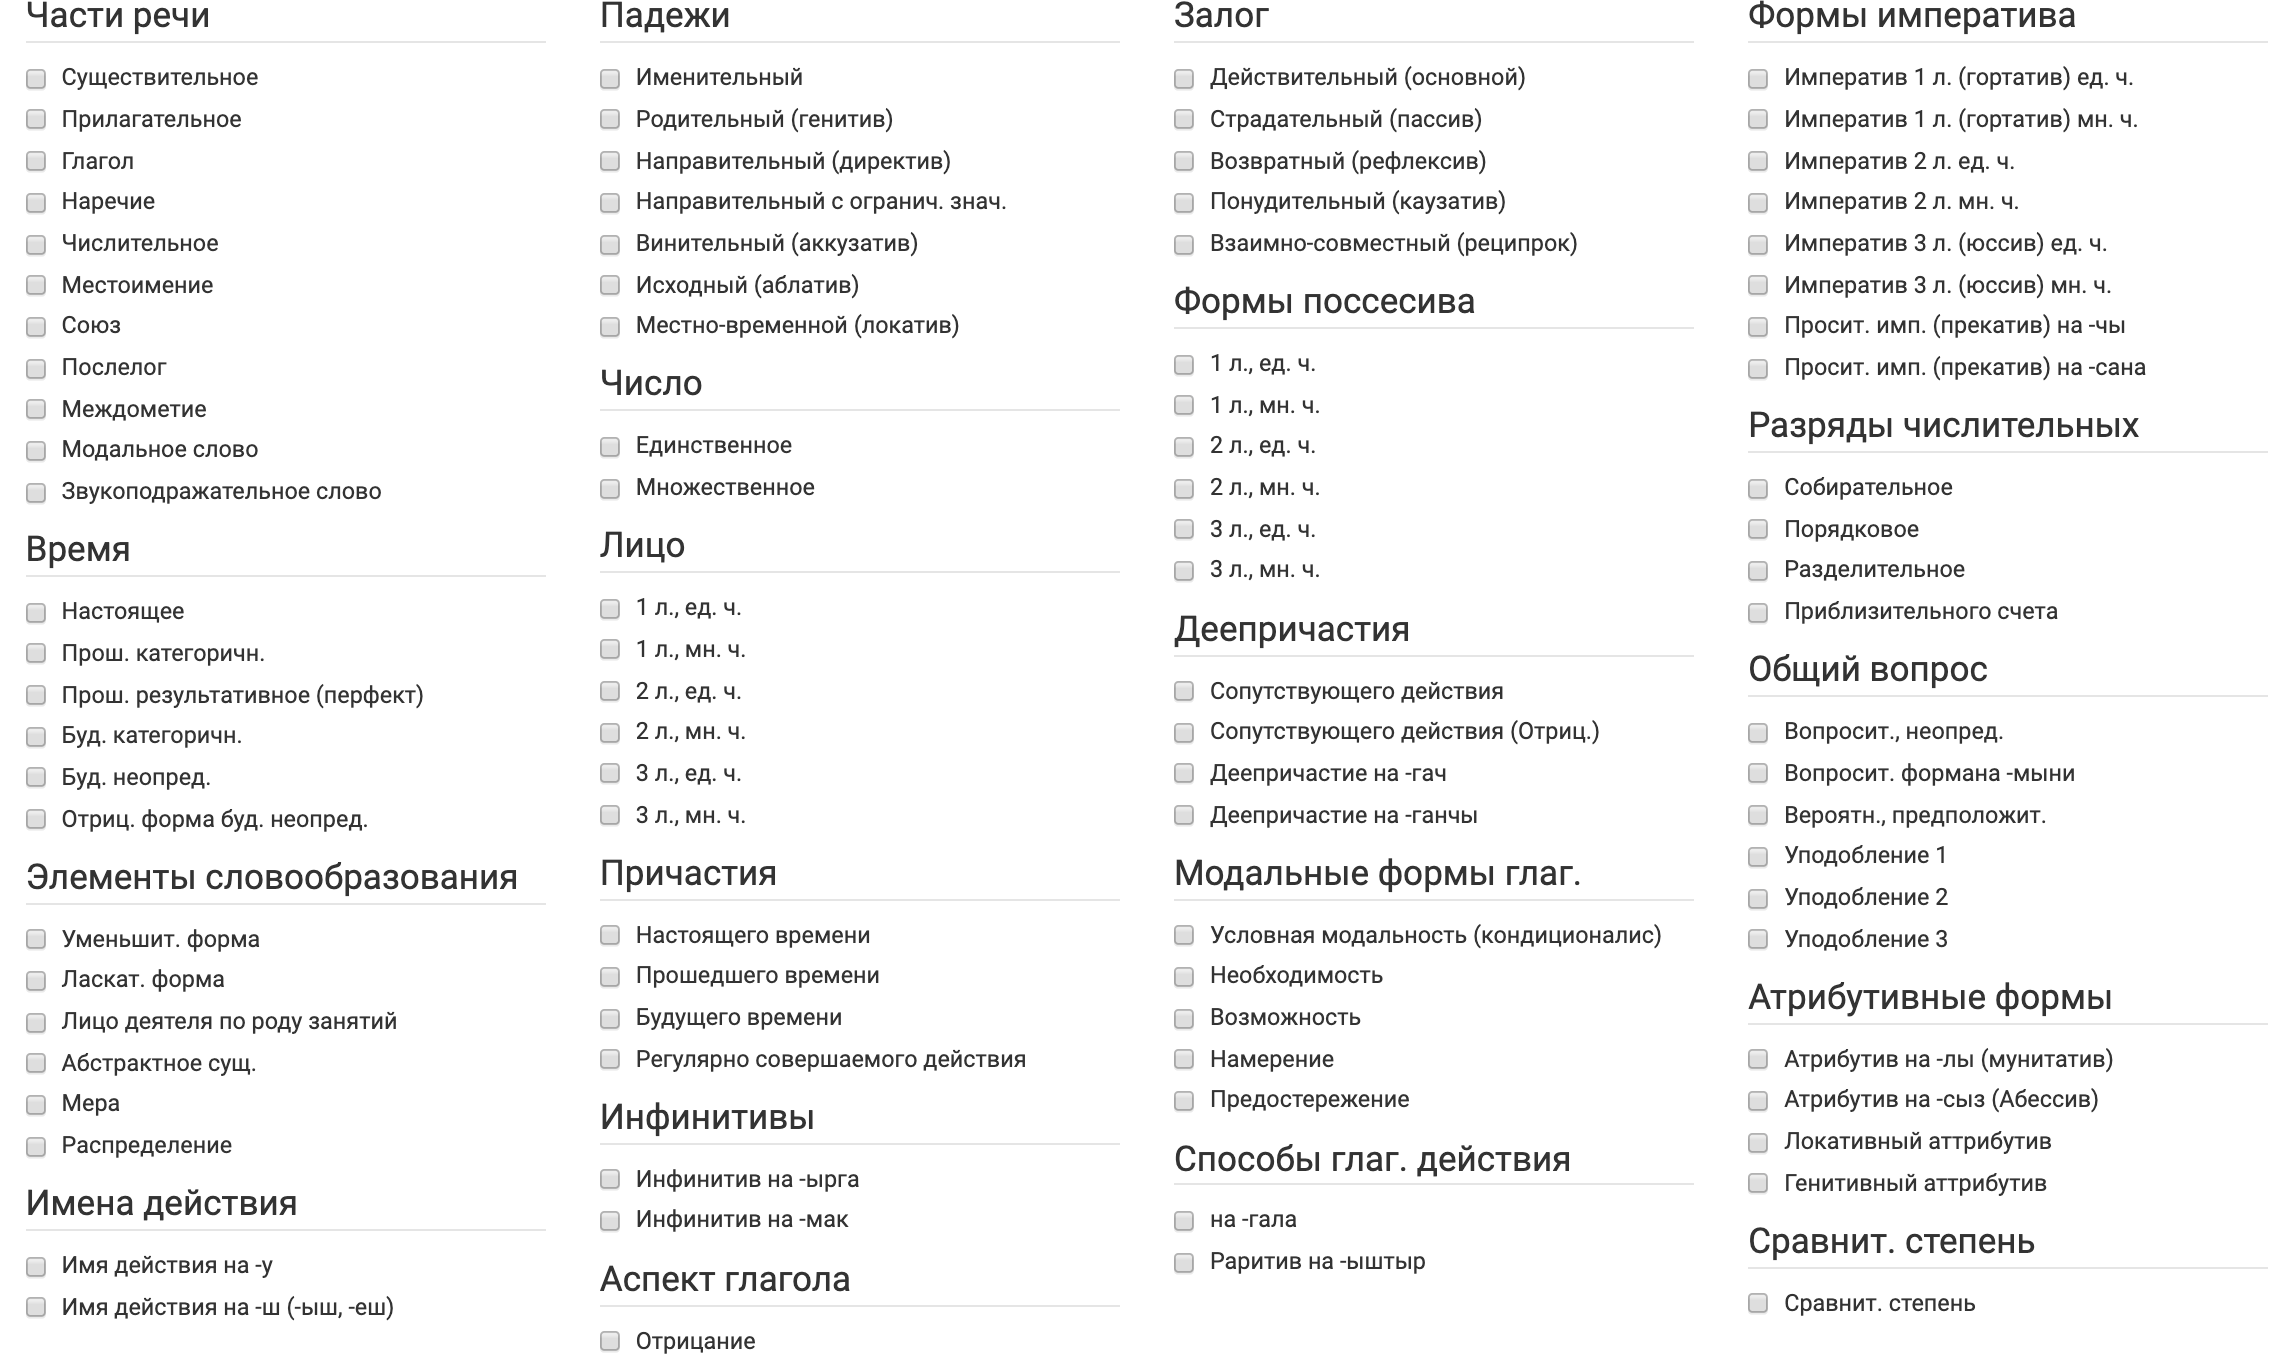
\includegraphics[width=\textwidth]{tugan_tel_1}
\label{fig:tugan_tel_1}
\end{figure}


Я связалась с Невзоровой по указанной в статье электронной почте, чтобы узнать подробности об их работе и попросить о сотрудничестве. Невзорова ответила на моё письмо и предоставила мне доступ к части корпуса, содержащей ~30 млн словоформ.

Корпус представляет собой .zip файл, состоящий из $7557$ .txt файлов, в общей сложности весом $1\ 183\ 023\ 978$ Б. Как уже упоминалось ранее, корпус Туган Тел автоматически размечен с помощью программного инструментарии PC-KIMMO. Разметка выглядит следующим образом (см. рис \ref{fig:sample_sent}). На нечетной строке написано слово, на следующей --- разметка слова. Знаки препинания тоже являются <<словоформами>>. Существует проблема с разделением текста на предложения, так как корпус не содержит никакой специальной разметки, обозначающей окончания предложений. Было принято решение разделять предложения по точкам, даже если это не самый точный способ разбиения.

\begin{figure}
\caption{Пример случайного предложения из корпуса Туган Тел}
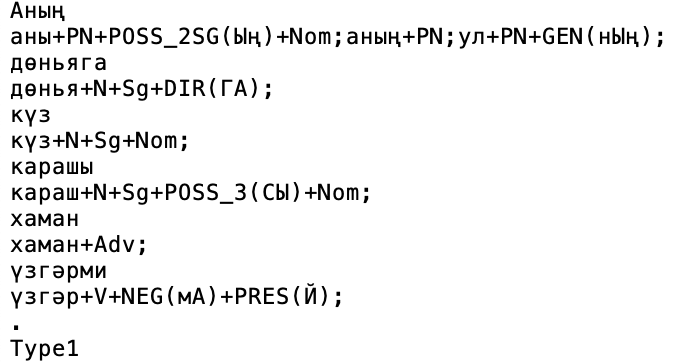
\includegraphics{sample_sent}
\label{fig:sample_sent}

Перевод: Его мировоззрение все ещё не меняется.
\end{figure}

Со всеми тегами морфоанализатора можно ознакомиться на сайте \\ \href{http://tatmorphan.pythonanywhere.com/morphan_tags}{tatmorphan.pythonanywhere.com}.

В тегах морфоанализатора присутствует тег PROP, который обозначает имена собственные. Для первой итерации было решено считать имена собственные именованными сущностями. Как можно заметить в примере на рис. \ref{fig:prop_sent}, в корпусе имена собственные иногда написаны с маленькой буквы, что говорит о том, что данные содержат ошибки.
Всего в текстах 30 753 824 слов, из них 534 514 это слова с атрибутом PROP, что составляет $1,7\%$ от всех слов. 

\begin{figure}
\caption{Пример предложения из корпуса Туган Тел с атрибутом PROP}
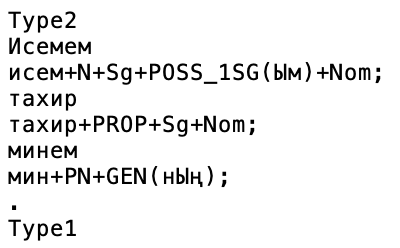
\includegraphics{pics/prop_sent}
\label{fig:prop_sent}

Перевод: меня зовут Тахир.
\end{figure}

\subsection{Татарская Википедия}

На данный момент татарская Википедия содержит $89\ 252$ статей, которые написаны как с помощью кириллической, так и с помощью латинской письменности. Данный раздел Википедии был открыт 15 сентября 2003 года и сначала функционировал исключительно на латинице, впоследствие статьи добавлялись с использованием обоих алфавитов; сейчас же достигнут консенсус об использовании единой системы категорий на кириллице, однако некоторые статьи до сих пор остаются латинизированными (примерно треть от всех имеющихся статей). Причин такой путаницы несколько. 

Во-первых, проблема алфавита в татарском языке стояла ещё со времен Советского Союза, т.к. до 1927 года использовалась арабская письменность, с 1927 по 1939 --- латинская письменность, а 5 мая 1939 года Президиум Верховного Совета Татарской АССР принял указ <<О переводе татарской письменности с латинизированного алфавита на алфавит на основе русской график>> и начал использоваться кириллический алфавит. Поскольку переход на другую письменность происходил принудительно, до сих пор ведутся дебаты о возвращении на латинский алфавит. В настоящий момент в республике Татарстан кириллица остаётся официальным алфавитом, однако стало допустимым использование латиницы и арабицы при обращении граждан в государственные органы и латиницы при транслитерации. Существует официальное соответствие данных трёх алфавитов.

Во-вторых, в 2000-x годах существовала проблема с записью текстов на компьютере, вызванная отсутствием букв дополнительной кириллицы в стандартных раскладках.

В связи с этим статьи на латинице пришлось конвертировать в кириллицу и в то же время случайно не перевести английские названия (например, ссылки). Данная процедура была проведена с помощью автоматического скрипта, поэтому возможны артефакты в виде, например, слова <<хттп>>.

\begin{figure}[H]
\begin{minipage}{\textwidth}
\caption{Статья <<Камский бассейновый округ>>}
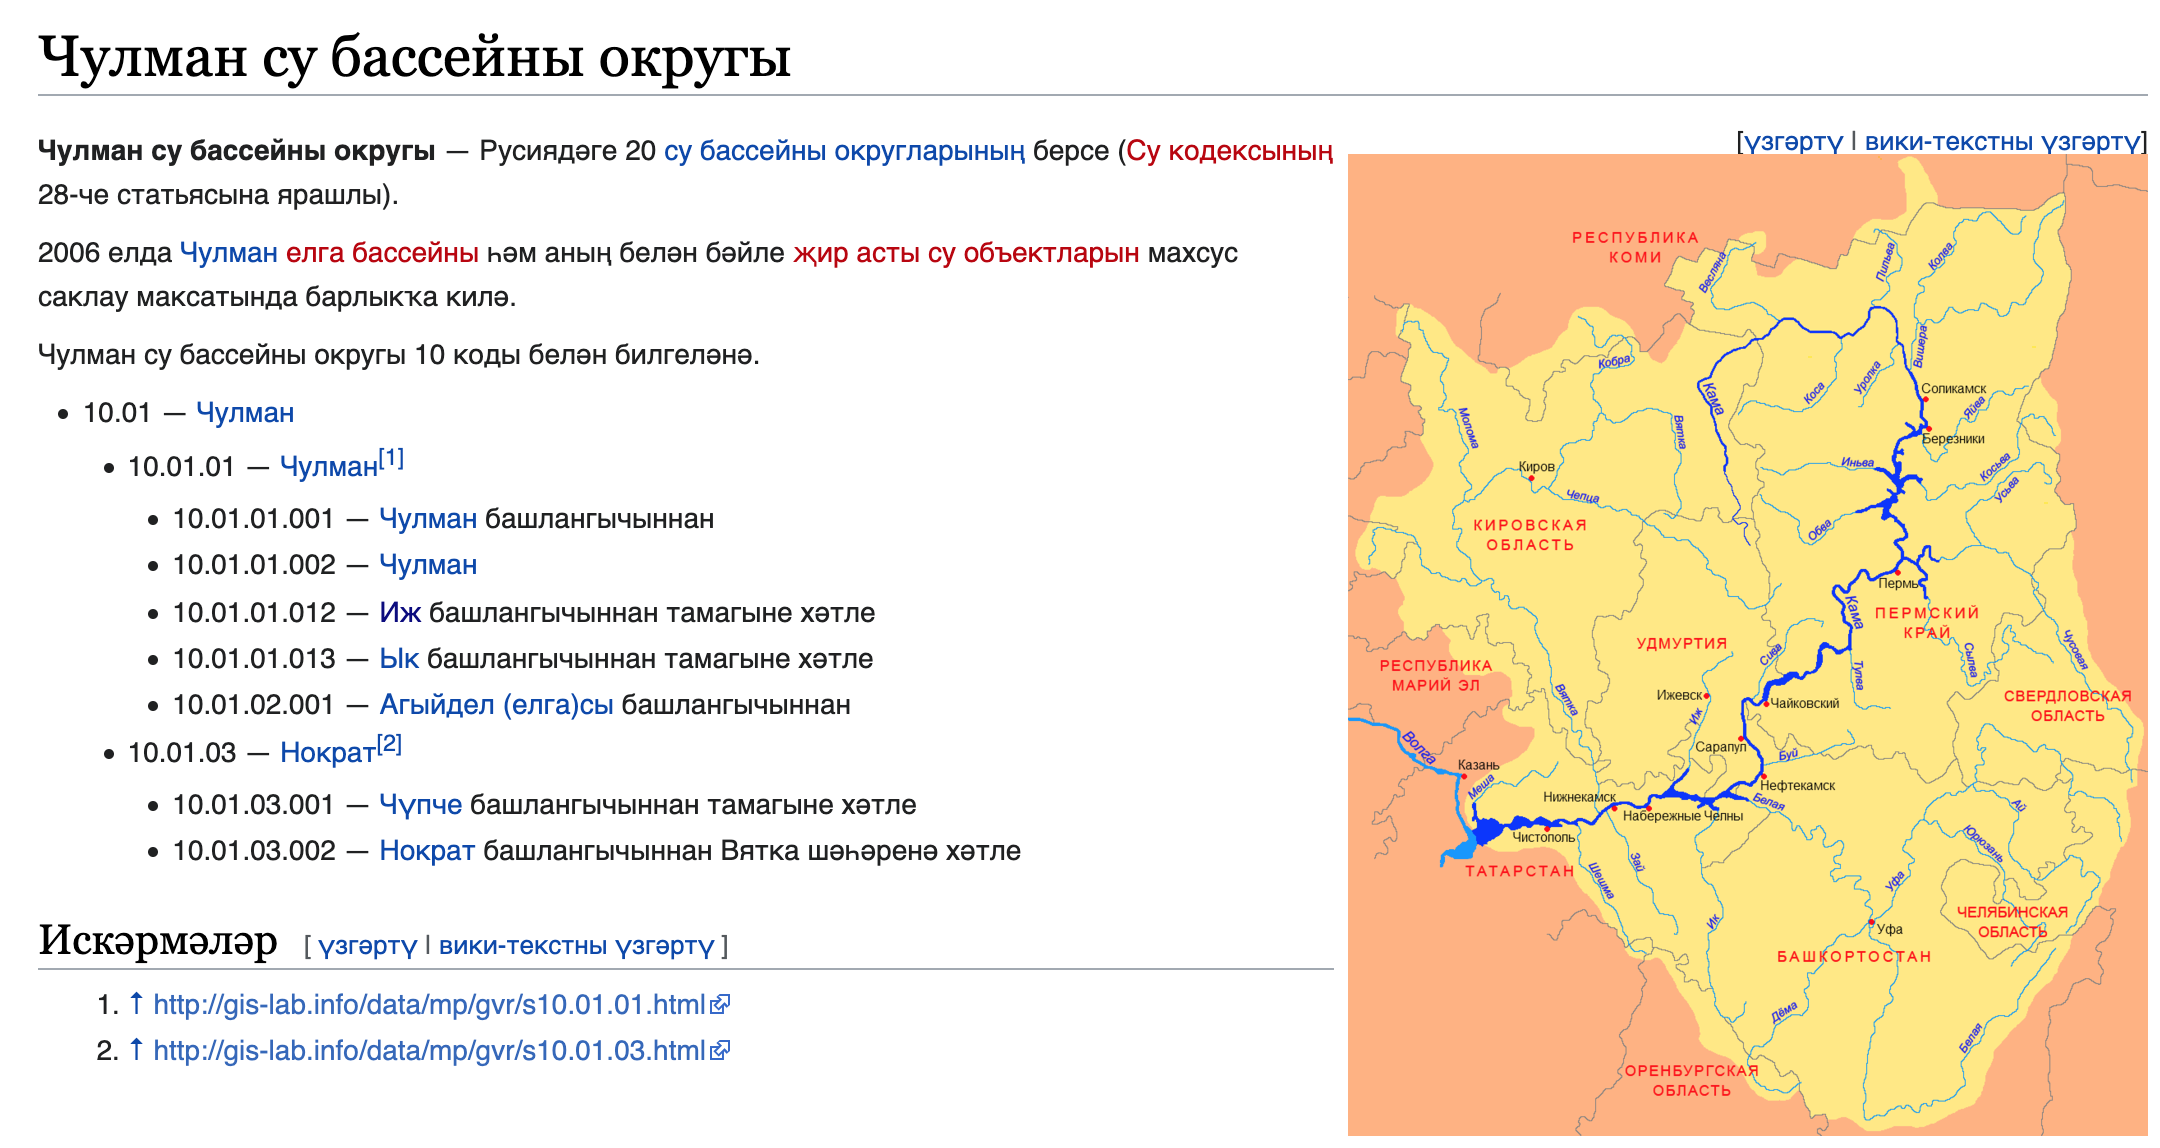
\includegraphics[width=\textwidth]{bassein_article}
\label{fig:bassein_article}
\end{minipage}

\begin{minipage}{\textwidth}
\caption{Пример сгенерированных статей из Википедии}
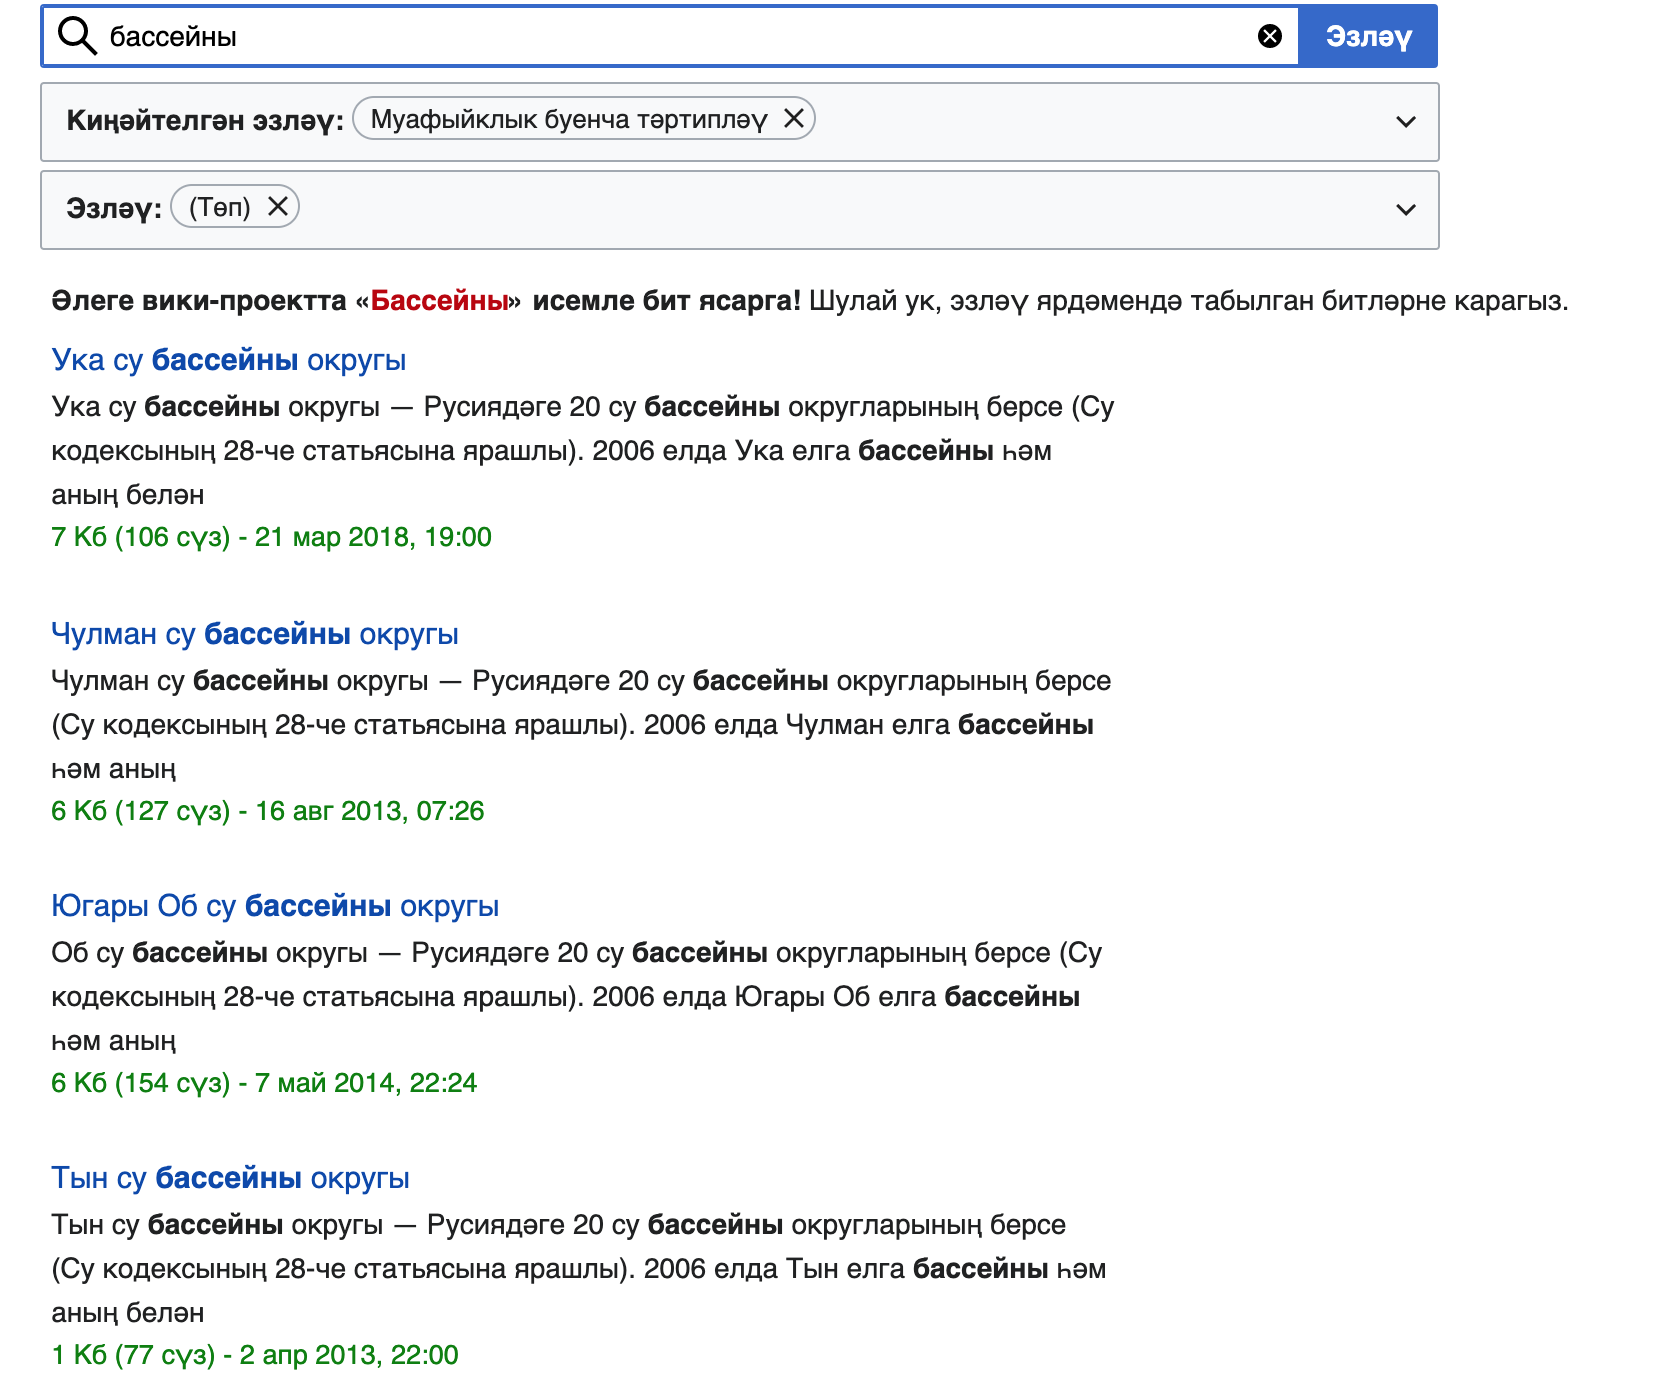
\includegraphics[width=\textwidth]{bassein_search}
\label{fig:bassein_search}
\end{minipage}
\end{figure}


Также важно отметить, что Википедия представляет собой набор статей, написанных в академическом стиле, что не вполне отражает разнообразие языка в различных сферах употребления; в этом аспекте Туган Тел гораздо лучше. В Википедии присутствуют автоматически сгенерированные статьи, это ухудшает качество текстов как корпуса для обучения, так как некоторые фразы становятся частотными не из-за того, что они действительно часто используются в языке, а из-за множества сгенерированных статей. Например, статьи про бассейновые округа (<<бассейны>> это не множественное число слова <<бассейн>>, а принадлежность к третьему лицу). Статья про Камский бассейновый округ (рис. \ref{fig:bassein_article}) и по тому же шаблону ещё много других статей про бассейновые округа (рис. \ref{fig:bassein_search}). 

Справедливости ради следует заметить, что в русской википедии они тоже сгенерированы автоматически. С другой стороны, Википедия имеет преимущество перед корпусом Туган Тел по количеству упоминаний географических названий.

\subsection{Разметка данных для обучения}

Первой итерацией было использование разметки PROP в корпусе Туган Тел, никакие другие теги морфоанализотора не использовались; Википедия не использовалась. 

Во второй итерации использовался воспроизведенный алгоритм Невзоровой, в качестве исходного корпуса для которого использовалась Википедия. На данных из Википедии был получен список n-грамм\footnote{Список n-грамм, обозначающих именованные сущности, предоставлен на github.com/ksemiya/NER\_in\_Tatar}, обозначающих именованные сущности по классам PER (персона), LOC (географический объект), ORG (организация) и MISC (названия языков) С помощью полученного списка была размечена Википедия с помощью сравнения n-грамм на точное равенство, в то время как Туган Тел никак не использовался при данной разметке и был отложен в качестве данных для оценивания.

Для разметки BIO был написан небольшой скрипт, с помощью которого вы можете также получить размеченные данные на своей локальной машине.


\subsection{Разметка данных для оценивания}

Автоматическая разметка не подходит для оценки результатов. Поэтому для оценивания воспроизведенного алгоритма Невзоровой и обученных моделей было принято решение разметить некоторое количество предложений вручную, в силу имеющихся знаний татарского языка. Предложения были выбраны из корпуса Туган Тел из соображений наличия в них хотя бы одной именованной сущности; для этого был использован алгоритм Невзоровой и если он определил наличие именованной сущности, то предложение добавлялось в список кандидатов на ручную разметку. Из полученного списка кандидатов предложения выбирались случайным образом, разметка алгоритмом Невзоровой удалялась до начала ручной разметки, чтобы не влиять на конечный результат. Получился тестовый набор данных golden-bio.txt \footnote{golden-bio.txt также предоставлен на github.com/ksemiya/NER\_in\_Tatar}, основанный на предложениях из корпуса Туган Тел (369 предложений).

\subsection{Проблемы с разметкой данных}

Как было описано и в статье Невзоровой, где исследователи глазами просматривали полученные результаты, отсеивали некорректные и улучшали свой алгоритм с помощью фильтров, так и в моей работе разметка данных происходила итеративно. Например, генерация статей про бассейны в Википедии была как раз выявлена в просмотре полученных результатов после разметки. Также выявлялись пробелы в алгоритме, например, некоторые географические названия, которые не попадали в список, были добавлены позже вручную. Для разметки тегом PER был использован справочник имён. Подводя итог, лучшей всё равно остаётся ручная разметка, а любая автоматическая разметка требует просмотра и последующей корректировки, возможно в несколько этапов, и это занимает очень много времени. С другой стороны, ручная разметка корпуса заняла бы ещё больше время.

\section{Обучение и тюнинг моделей}

\subsection{BiLSTM-CRF}

Была использована модель BiLSTM-CRF из статьи <<A Neural Layered Model for Nested Named Entity Recognition>> \cite{ju-etal-2018-neural}. Она использует разметку BIO, как и многие другие модели для извлечения именованных сущностей. Архитектура модели изображена на рис. \ref{fig:BiLSTMCRF}

\begin{figure}[H]
\caption{Архитектура модели BiLSTM-CRF, рис. из статьи \cite{ju-etal-2018-neural}}
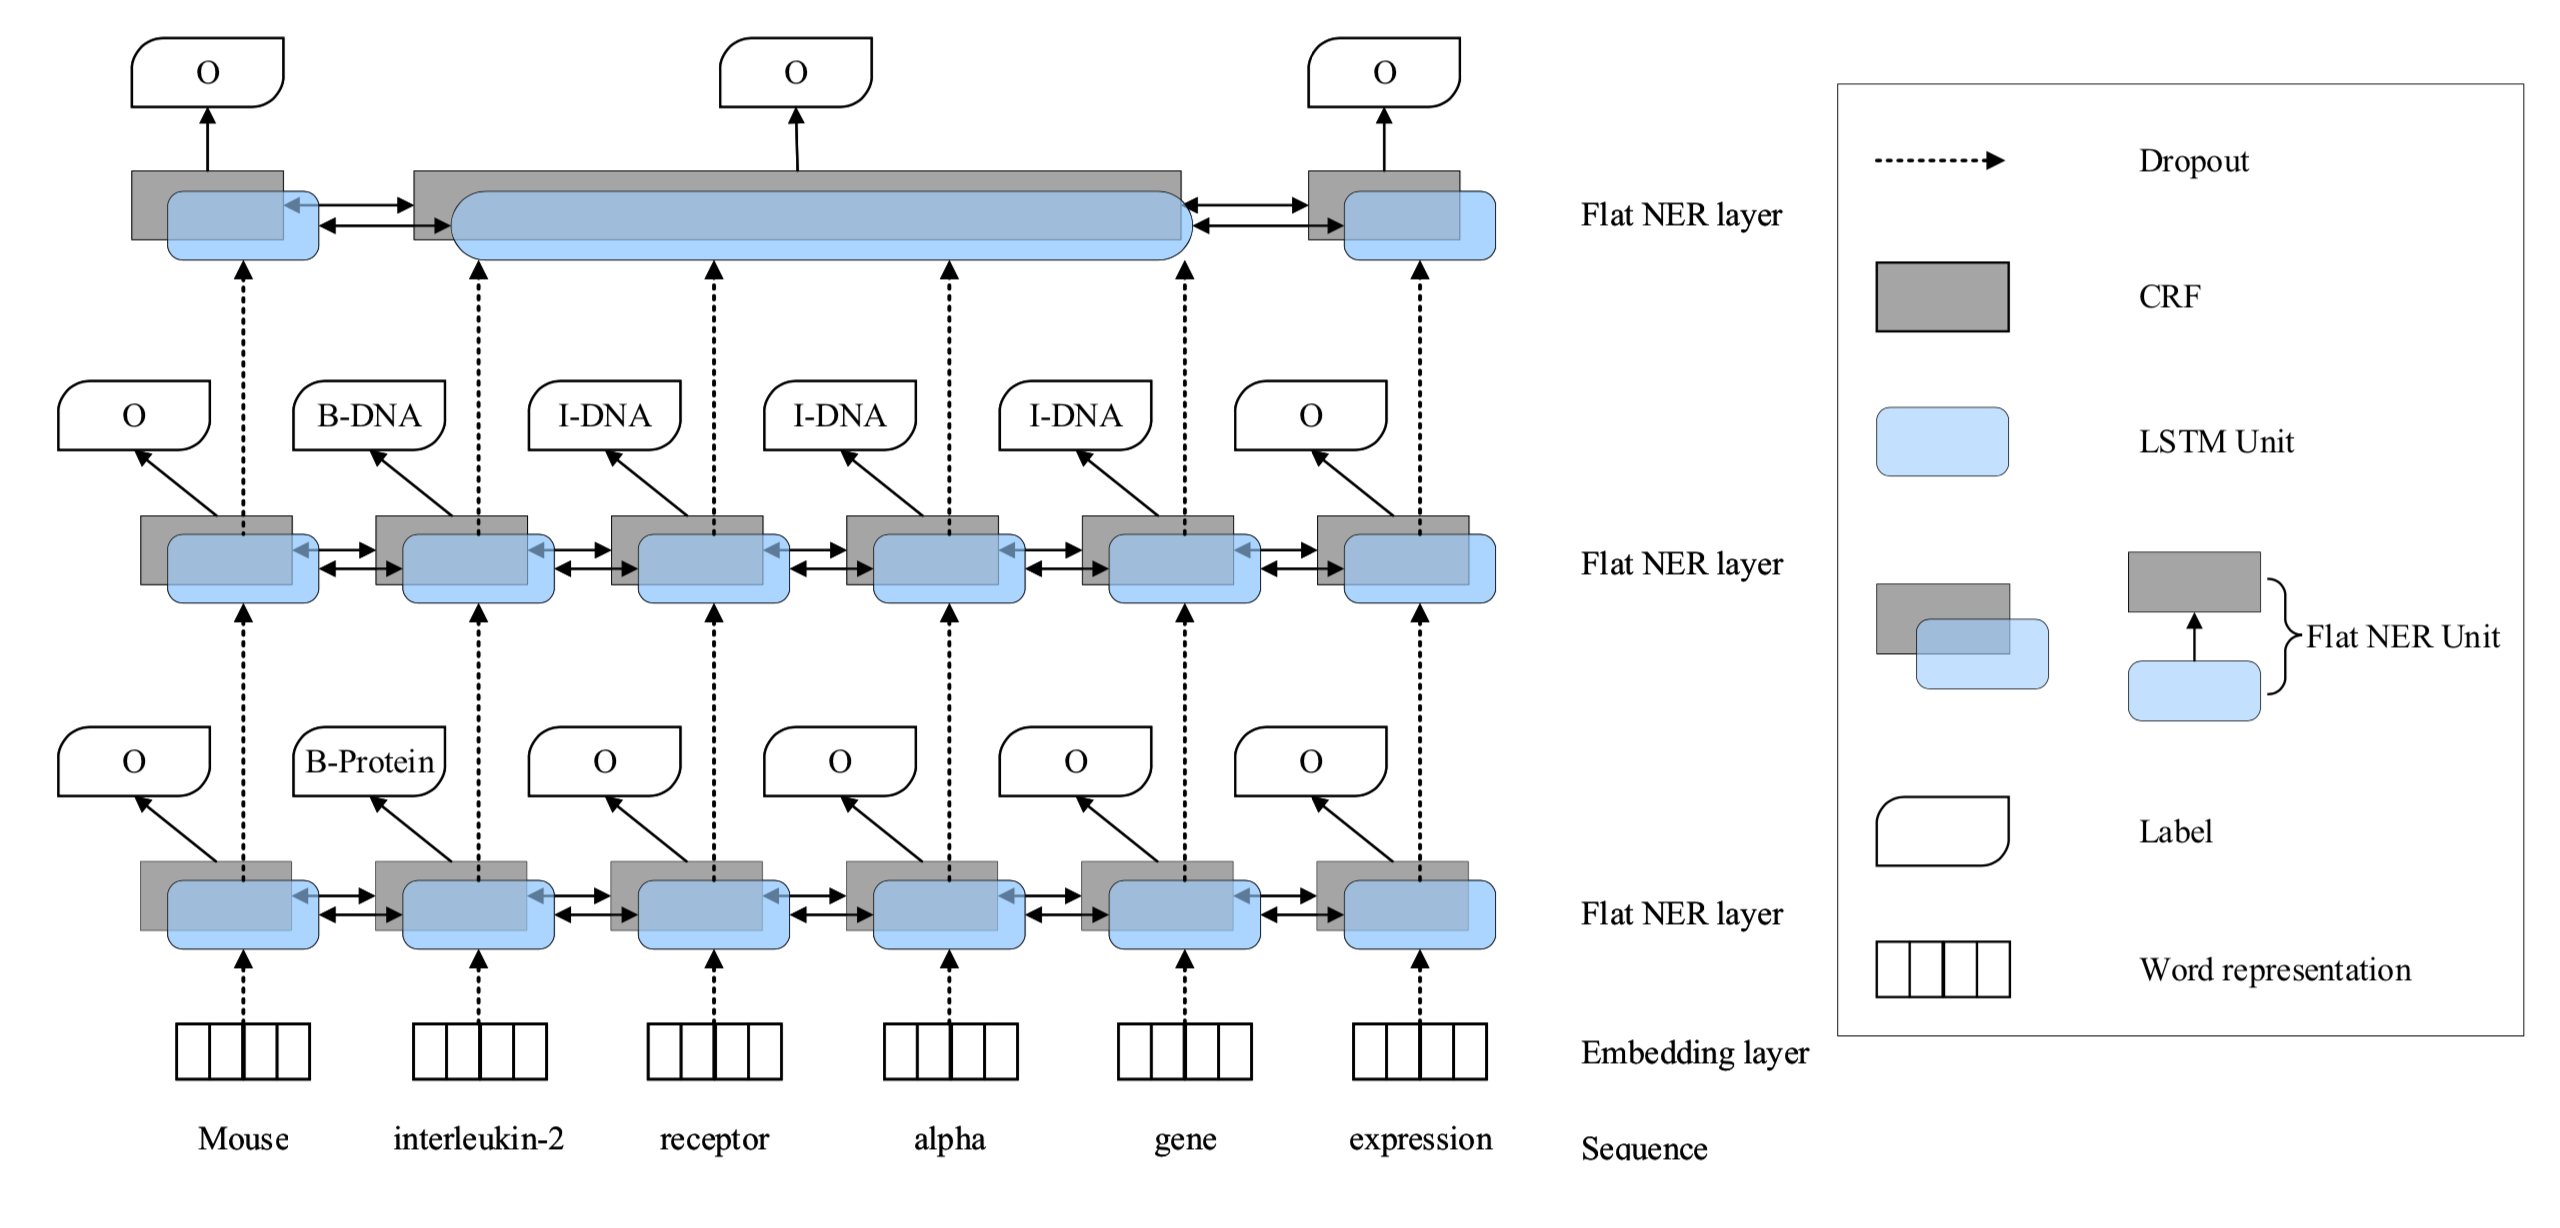
\includegraphics[width=\textwidth]{BiLSTMCRF}
\label{fig:BiLSTMCRF}
\end{figure}


Была возможность запустить модель только на локальной не очень мощной машине, поэтому пришлось обучать модель не на всех данных, а только на части.

Первая итерация на данных Туган Тел. Результат обучения, в данных два тега: O и PROP.

\vspace{1cm}

\begin{table}[h]
\begin{tabular}{ | l | l | l | l | l | l |}
\hline
Precision  &   Recall   &  F-score   \\

\hline
99.768     & 90.727     & 95.033      \\
\hline
\end{tabular}
\caption{Обучение BiLSTM-CRF на первых данных}
\end{table}

\vspace{1cm}

Была сделана демонстрация работы модели в виде сайта, запускающегося на локальной машине, но самые простые примеры не из тестового набора выявили большие несовершенства данной модели --- она не извлекала именованные сущности в самых простых предложениях, поэтому в итоге было принято решение отказаться от её использования. %TODO скриншот
Как можно понять, цифры выше показывают способность модели обучаться на данных (и модель действительно обучается хорошо, выборка разделяется на тестовую и валидационную и всегда показывает хороший результат), но проблема в том, что сами данные очень низкого качества --- и эту проблему модель, увы, исправить не может.

Вторая итерация обучения была произведена на Википедии, размеченной с помощью списка n-грамм, полученных с помощью алгоритма Невзоровой. В тренировочном наборе были оставлены только те предложения, где есть хотя бы одна именованная сущность.

Результат обучения, в данных 9 тегов:
B-LOC
B-MISC
B-ORG
B-PER
I-LOC
I-MISC
I-ORG
I-PER
O
\vspace{1cm}

\begin{table}[h]
\begin{tabular}{| l | l | l | l | l | l |}
\hline
Precision  &   Recall   &  F-score   \\

\hline
                89.421     & 86.825     & 88.104          \\
\hline
\end{tabular}
\caption{Обучение BiLSTM-CRF на улучшенных данных}
\end{table}
\vspace{1cm}
\subsection{BERT}

\cite{DBLP:journals/corr/abs-1810-04805} Одна из самых известных моделей на сегодняшний день, показала лучшие результаты на классических данных CoNLL 2003 (см. обзор литературы).

Для решения моей задачи была использована библиотека Hugging face \cite{Wolf2019HuggingFacesTS} и претренированная модель bert-base-multilingual-cased, которая обучена на чувствительных к регистру данных из 104-х наибольших Википедий. Данная модель включает в себя и татарский язык (беглый взгляд по токенам показал, что действительно есть как и кириллические, так и латинские токены на татарском языке). 

При обучении модели возникли проблемы с размером корпуса данных. Из-за особенностей реализации обучения модели BERT в HuggingFace, библиотека не была способна сохранить все признаки полностью. Особенность была связана с реализацией загрузки данных в библиотеке. Ей нужно было сохранить все данные в виде признаков PyTorch. Обучение удалось произвести только лишь на $1/3$ всех доступных данных.

Результат обучения, в данных два тега: O и PROP.

\vspace{1cm}
\begin{table}[h]
\begin{tabular}{| l | l | l |}
\hline
Precision  &   Recall   &  F-score     \\

\hline
97.447     & 94.585    & 95.995        \\
\hline
\end{tabular}
\caption{Обучение BERT на первых данных}
\end{table}

\vspace{1cm}

Один в один повторение истории с BiLSTM-CRF --- сами по себе цифры очень многообещающие, модель обучилась прекрасно, но на деле они показывают всего лишь натренированность модели на плохих начальных данных. Модель в итоге не работает на простых примерах, придуманных из головы. Было принято решение от этой модели отказаться. %TODO скриншот

Вторая итерация обучения была произведена на Википедии, размеченной с помощью списка n-грамм, полученных с помощью алгоритма Невзоровой. В тренировочном наборе были оставлены только те предложения, где есть хотя бы одна именованная сущность.

Результат обучения, в данных 9 тегов:
B-LOC
B-MISC
B-ORG
B-PER
I-LOC
I-MISC
I-ORG
I-PER
O

\vspace{1cm}
\begin{table}[h]
\begin{tabular}{| l | l | l |}
\hline
Precision  &   Recall   &  F-score     \\

\hline
88.853    & 92.377    & 90.581        \\
\hline
\end{tabular}
\caption{Обучение BERT на улучшенных данных}
\end{table}

 \vspace{1cm}

Как видно, результаты заметно ухудшились, что неудивительно, ведь классов стало в $4.5$ раза больше.

Однако все эти результаты всего лишь показывают, как хорошо модель обучилась предсказывать результаты на имеющихся данных. Чтобы проверить её реальную способность извлекать именованные сущности, необходимо проверить предсказания на <<золотых>> данных, размеченных вручную, про которые мы с высокой точностью знаем, что они правильные.


\section{Воспроизведение алгоритма из статьи Невзоровой}

Было принято решение воспроизвести алгоритм из статьи Невзоровой и др. \cite{Nevzorova} по двум причинам.

\begin{enumerate}
\item Чтобы была возможность сравнивать результаты.
\item Чтобы разметить данные эффективно и, по возможности, хорошо.
\end{enumerate}

%Обе цели были достигнуты и теперь я имею возможность рассказать вам о проблемах, с которыми я столкнулась во время работы и результатах, полученных в итоге.

Воспроизводить алгоритм по описанию в статье было нетривиально, поэтому, если будут желающие воспроизвести его ещё раз, то я рекомендую описание, которое я дала выше в разделе обзор литературы.

Как было сказано ранее, у меня не было доступа к системе <<корпус-менеджер>> Туган Тел \cite{tugan_tel}, поэтому воспроизвести алгоритм в точности не удалось. Попытка приблизиться к результату состояла в том, чтобы использовать в качестве начального слова все возможные формы слова, а не только слово само, т.е. частично сделать работу морфоанализатора вручную. Однако возможность делать запросы по каким-то морфологическим параметром не была реализована.

Несмотря на все вышеописанные трудности, алгоритм сработал достаточно хорошо, хотя и, как и сказано в работе Невзоровой и др., требовалась значительная ручная чистка полученных данных.

Ручная чистка состояла в просмотре полученных именованных сущностей и исправление п возможности не точечно, а <<широкими мазками>> --- добавлением новых начальных слов для поискового запроса или удалением всех очевидно некорректных n-грамм одним вызовом команды grep. Например, по слову <<министрлыгы>> (министерство) появилось множество n-грамм, которые начинались с союза <<һәм>> (и). Это некорректные n-граммы, но удалить их все было достаточно легко. 

Также помимо слов, представленных в работе Невзоровой и др. в качестве начальных, были использованы и другие слова, такие как географические объекты: <<елга>> (река), <<шәһәр>> (город), <<авыл>> (село), <<өлкә>> (область) и др., организации:  <<академияс>> (академия), <<идарә>> (администрация), <<институт>> (институт) и др., персоны: <<абый>> (старший брат), <<апа>> (старшая сестра) и др. (в татарском языке принято называть родственников, например, Ильдар абый, Сания апа, поэтому это часто встречающийся шаблон).

В результате получился список из ~30 тысяч именованных сущностей, который доступен на моём github. %TODO более точная информация
Он может пригодиться людям, которые будут продолжать работу в данном направлении для разметки собственных корпусов или извлечения именованных сущностей. 

\section{Демонстрация полученных результатов}

Был сделан демонстрационный http-сервер, работающий локально на рабочей станции, с помощью которого можно проверить модель на работоспособность.

%TODO новые скриншоты

\begin{figure}[H]
\caption{Старший научный сотрудник историческго института имени Мержани}
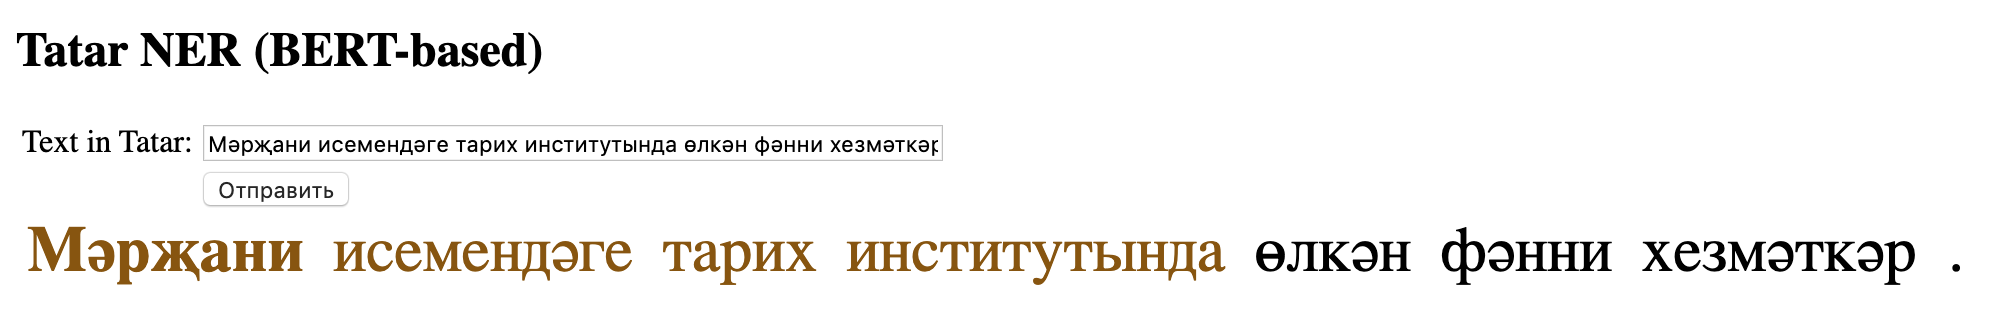
\includegraphics[width=\textwidth]{BERT_samp_1}
Всё распознано корректно, категория ORG
\label{fig:BERT_samp_1}
\end{figure}
\begin{figure}[H]
\caption{Зовут меня Ксения}
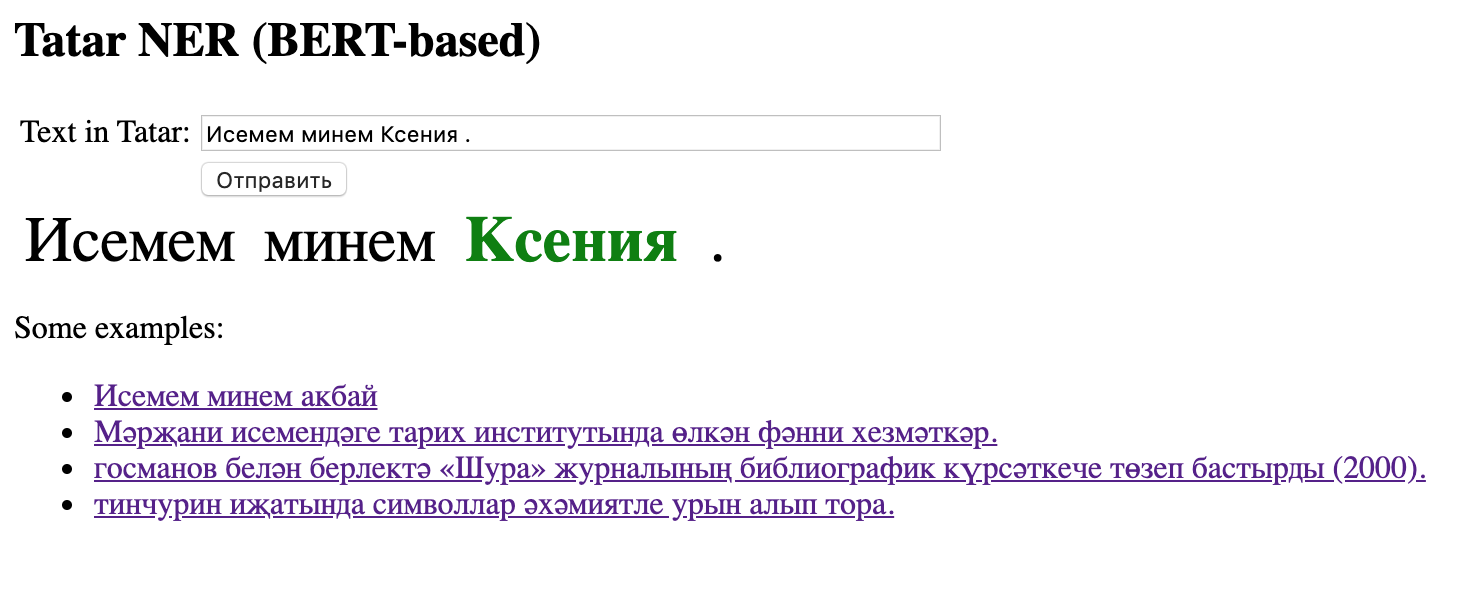
\includegraphics[width=\textwidth]{BERT_samp_2}
Всё распознано корректно, категория PER
\label{fig:BERT_samp_2}
\end{figure}
\begin{figure}[H]
\caption{Он прочитал решение на русском языке}
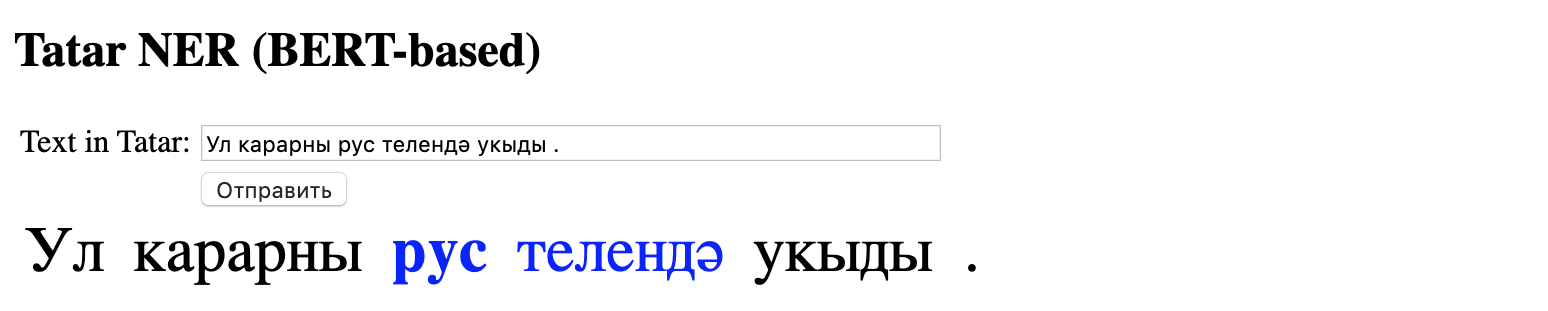
\includegraphics[width=\textwidth]{BERT_samp_3}
Всё распознано корректно, категория MISC
\label{fig:BERT_samp_3}
\end{figure}
\begin{figure}[H]
\caption{Празднование состоится в селе Асан Дюртюлинского района}
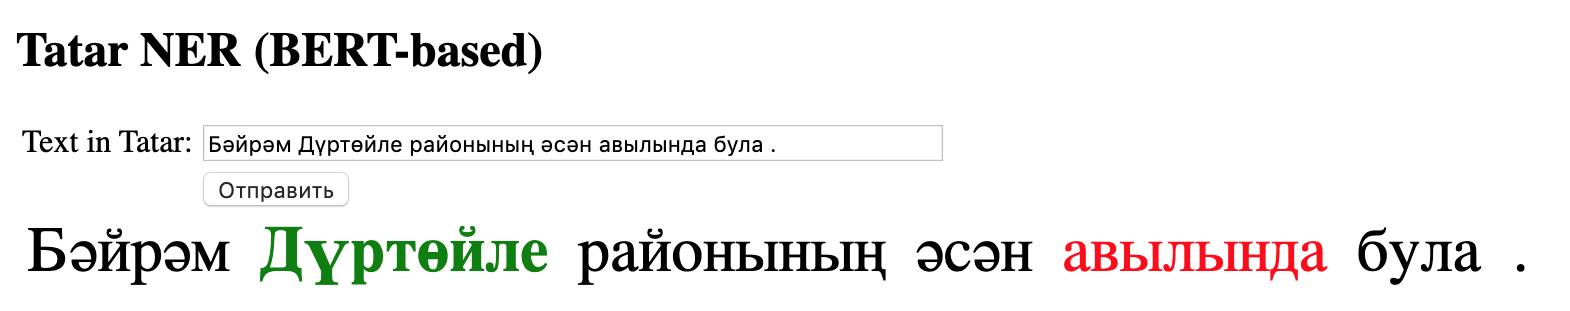
\includegraphics[width=\textwidth]{BERT_samp_4}
Не распознано имя села, хотя само понятие <<село>> распознано как категория LOC. <<Дюртюлиский>> ошибочно распознано как имя, <<район>> должно входить в название района.
\label{fig:BERT_samp_4}
\end{figure}



\section{Сравнение результатов}

Отдельной задачей стоял вопрос, как сравнить полученные результаты с предыдущими результатами в данной области. Было принято решение разметить некоторое количество предложений вручную, чтобы иметь качественные <<золотые>> данные, про которые было бы известно, что вероятность ошибок в них гораздо ниже, чем в автоматически размеченных. Такая разметка была получена и следующим этапом воспроизведенный алгоритм Невзоровой, ВiLSTM-CRF и BERT (последние два обученные на датасете, основанном на Википедии) были запущены на этих данных. Теперь полученные результаты допустимо сравнивать между собой, поскольку они <<в равном положении>> и выполняют одинаковую задачу. Но нужно заметить, что модели BiLSTM-CRF и BERT были обучены на данных, размеченных по методу Невзоровой и др., поэтому результаты моделей не полностью независимы.

Как видно из цифр таблиц [\ref{table:Nevzorova_res_1}], [\ref{t}], [\ref{table:average}], разметка данных с помощью алгоритма Невзоровой и др. далеко не идеальная, и модели выучили ровно столько, сколько данные могли им дать (однако у меня была надежда, что модели выучат больше, чем им дали на вход; для этого они обучались на данных, которые не содержали в себе <<пустые>> предложения, чтобы не учить их определять данные без меток). 

\newpage

\begin{table}[h!]
\begin{tabular}{| l | l | l | l | l |}
\hline


 category &precision  &  recall & \textbf{f1-score} &  total\\
 \hline
 PER& 0.53&0.63&\textbf{0.58}& 374 \\
  \hline
 LOC& 0.50&0.05&\textbf{0.09}&  78 \\
  \hline
 ORG& 0.40&0.10&\textbf{0.15}&  21 \\ 
  \hline
 MISC& 0.83&0.62&\textbf{0.71}&   8 \\ 
 \hline
 \hline

 macro avg& 0.52&0.51&\textbf{0.48}& 481 \\
\hline
\end{tabular}

\caption{Результаты алгоритма Невзоровой}
\label{table:Nevzorova_res_1}
\end{table}

\hfill
\begin{table}[h!]
\begin{subtable}[h]{0.4\textwidth}

\begin{tabular}{| l | l | l | l | l |}
\hline

 category &precision  &  recall & \textbf{f1-score} &  total\\
\hline
PER &  0.53 & 0.60 & \textbf{0.56} &  374 \\ 
\hline
LOC &  0.50 & 0.05 & \textbf{0.09} &   78 \\ 
\hline
ORG &  0.33 & 0.10 & \textbf{0.15} &   21 \\
\hline
MISC &  0.56 & 0.62 & \textbf{0.59} &   8 \\
\hline
\hline

 macro avg &  0.52 & 0.49 & \textbf{0.47} &  481 \\
\hline
\end{tabular}

\caption{Результаты модели BERT}
%\label{table:BERT_res_1}
\end{subtable}

\hfill

\begin{subtable}[h]{0.4\textwidth}

\begin{tabular}{| l | l | l | l | l |}
\hline

 category &precision  &  recall & \textbf{f1-score} &  total\\
\hline
PER &  0.52 & 0.44 & \textbf{0.48} &  374 \\ 
\hline
LOC &  1.00 & 0.03 & \textbf{0.05} &   78 \\ 
\hline
ORG &  0.33 & 0.10 & \textbf{0.15} &   21 \\
\hline
MISC &  0.44 & 0.50 & \textbf{0.47} &   8 \\
\hline
\hline

 macro avg &  0.59 & 0.36 & \textbf{0.39} &  481 \\
\hline


\end{tabular}

\caption{Результаты модели Bi-LSTM-CRF}
%\label{table:BiLSTMCRF_res_1}
\end{subtable}

\caption{Результаты нейросетевых моделей}
\label{t}
\end{table}


\begin{table}[h!]

\begin{tabular}{| l | l | l | l |}
\hline

model &precision  &  recall & \textbf{macro f1} \\
\hline
Алгоритм разметки данных & 0.52 & 0.51& \textbf{0.48} \\ 
\hline
BERT &  0.52 & 0.49 & \textbf{0.47} \\ 
\hline
BiLSTM-CRF &  0.59 & 0.36 & \textbf{0.39} \\
\hline
\end{tabular}

\caption{Сравнительная таблица,  macro avg}
\label{table:average}

\end{table}

%Результаты тестирования модели BERT на <<золотых>> данных приведены в таблице \ref{table:BERT_res_1}


%Результаты тестирования модели BiLSTM-CRF на <<золотых>> данных приведены в таблице \ref{table:BiLSTMCRF_res_1} пока таблицы нет, но скоро будет, и моё предположение таково, что он будет ещё хуже, чем BERT. Но даже если сравнимо, то точно не лучше, чем алгоритм Невзоровой.




\newpage

\section{Выводы}

\begin{enumerate}
\item Воспроизведен алгоритм из статьи Невзоровой и др., он показал свою работоспособность и его можно использовать в дальнейшем. %ограничения
\item Получен набор n-грамм именованных сущностей и размеченный корпус, с которыми можно будет работать в дальнейшем.
\item Получены модели, предсказывающие именованные сущности, но результаты этих моделей из-за качества данных оставляют желать лучшего.
\item Лучшие известные модели действительно работают хорошо и на татарском языке, обучаясь на данных настолько, насколько данные это позволяют, но увы, ничего сверх этого получить от них не удалось. 
\item Всё зависит от того, насколько хорошо размечены данные, поэтому в будущих работах нужно лучше разметить данные, количество доступных данных было вполне достаточным для обучения моделей.
\end{enumerate}
























    \section{Заключение}

Проведена большая хорошая работа, получены хорошие результаты, статья Невзоровой должна была называться не так пафосно, но они тоже молодцы, хорошую работу сделали.

Можно будет сотрудничать с Академией наук Республики Татарстан и дальше двигать направление распознавания именованных сущностей, пробовать новые модели не только распознавания, но также и разметки данных, поскольку с каждым годом корпус Туган тел становится объемнее. Использовать в качестве признаков морфологические параметры и не только. Направлений для работы много и это хорошее поле для дальнейших исследований.
    
    \addcontentsline{toc}{chapter}{Список литературы}
    \bibliographystyle{utf8gost705u}  %% стилевой файл для оформления по ГОСТу
    \bibliography{biblio}     %% имя библиографической базы (bib-файла)


\end{document}
